\documentclass[a4paper]{memoir}
\usepackage{lecture-notes}
\usepackage{float}



\begin{document}
\beginLectureNotes

\newpage
\section{Préambule : Régression linéaire, régression ridge et LASSO}
\subsection{Calculs préliminaires}
Soient $f_w$ la fonction de prédiction et $\hat{y}$ l'ensemble des vrais labels de la base d'apprentissage.


\subsubsection{Régularisation L2}
On souhaite minimiser la fonction de coût suivante :
\begin{equation*}
L_2(w) = \frac{1}{2N} \sum_{i=1}^{N}{\big(\hat{y_i} - f_w(x_i)\big)^2} + \alpha||w||_2^2
\end{equation*}

On va donc l'optimiser par descente de gradient, en utilisant le gradient suivant :
\begin{equation*}
\derivative{L_2}{w}{} = \frac{1}{N} \sum_{i=1}^{N}{\big(\hat{y_i} - f_w(x_i)\big)x_i} + 2\alpha w
\end{equation*}


\subsubsection{Régularisation L1}
On souhaite minimiser la fonction de coût suivante :
\begin{equation*}
L_1(w) = \frac{1}{2N} \sum_{i=1}^{N}{\big(\hat{y_i} - f_w(x_i)\big)^2} + \alpha||w||_1
\end{equation*}

On va donc l'optimiser par descente de gradient, en utilisant le gradient suivant :
\begin{equation*}
\derivative{L_1}{w}{} = \frac{1}{N} \sum_{i=1}^{N}{\big(\hat{y_i} - f_w(x_i)\big)x_i} + \alpha \cdot sign(w)
\end{equation*}


\subsection{Description du protocole}
Le classifieur utilisé est, comme décrit dans l'énoncé, une simple \textbf{régression linéaire} adaptée à la classification binaire par la méthode du \textbf{plug-in}. Nous comparerons différentes fonctions de coût : \textbf{MSE}, \textbf{régularisation $L_2$} et \textbf{régularisation $L_1$}, ainsi que plusieurs valeurs du coefficient $\alpha$. De plus, nous comparons aussi nos résultats avec les implémentations \textit{LinearRegression} et \textit{Lasso} de la bibliothèque \textbf{sklearn} et adaptées par la \textit{méthode du plug-in}.\\

La base de données \textbf{USPS} étant déjà séparée en une base d'apprentissage et une base de test, nous pouvons facilement calculer le score obtenu sur cette même base de test. Nous proposons de comparer les résultats obtenus en classifiant \textbf{chaque classe contre chaque autre} dans un premier temps, puis dans du \textbf{1 contre tous} par la suite. Enfin, nous étudierons l'apparence du vecteur de poids obtenu par chaque méthode de classification en comptant le \textbf{nombre de poids nuls} ainsi que la \textbf{moyenne de la valeur absolue des poids}.


\subsection{Analyse des résultats}
\begin{table}[H]
  \centering
  \renewcommand{\arraystretch}{1.5}
  \begin{tabular}{|l|c|c|c|}
     \hline
     \thead{Classifieur} & \thead{Score moyen} & \thead{Nombre de $0$} & \thead{moyenne de $|w|$} \\ \hline \hline
     \textbf{Régression linéaire plug-in, $MSE$}                & 0.5290 & 0     & 0.25045    \\ \hline
     \textbf{Régression linéaire plug-in, $L_2$, $\alpha=0.00$} & 0.4853 & 0     & 0.24862    \\ \hline
     \textbf{Régression linéaire plug-in, $L_2$, $\alpha=0.25$} & 0.5179 & 0     & 0.00285    \\ \hline
     \textbf{Régression linéaire plug-in, $L_2$, $\alpha=0.50$} & 0.5256 & 0     & 0.00308    \\ \hline
     \textbf{Régression linéaire plug-in, $L_2$, $\alpha=0.75$} & 0.5276 & 0     & 0.00265    \\ \hline
     \textbf{Régression linéaire plug-in, $L_2$, $\alpha=1.00$} & 0.5095 & 0     & 0.00258    \\ \hline
     \textbf{Régression linéaire plug-in, $L_1$, $\alpha=0.00$} & 0.5638 & 0     & 0.24974    \\ \hline
     \textbf{Régression linéaire plug-in, $L_1$, $\alpha=0.25$} & 0.5179 & 0     & 0.00387    \\ \hline
     \textbf{Régression linéaire plug-in, $L_1$, $\alpha=0.50$} & 0.5016 & 0     & 0.00473    \\ \hline
     \textbf{Régression linéaire plug-in, $L_1$, $\alpha=0.75$} & 0.5225 & 0     & 0.00573    \\ \hline
     \textbf{Régression linéaire plug-in, $L_1$, $\alpha=1.00$} & 0.5229 & 0     & 0.00642    \\ \hline
     \textbf{sklearn.LinearRegression plug-in, $\alpha=1.00$}   & 0.9732 & 17    & 99305970.4 \\ \hline
     \textbf{sklearn.Lasso plug-in, $\alpha=0.10$}              & 0.9535 & 10832 & 0.00444    \\ \hline
     \textbf{sklearn.Lasso plug-in, $\alpha=1.00$}              & 0.5607 & 11520 & 0.00000    \\ \hline
  \end{tabular}
  \small{Résultats obtenus pour chaque classifieur sur la base \textbf{USPS} en \textbf{classe contre classe}}
\end{table}

\begin{table}[H]
  \centering
  \renewcommand{\arraystretch}{1.5}
  \begin{tabular}{|l|c|c|c|}
     \hline
     \thead{Classifieur} & \thead{Score moyen} & \thead{Nombre de $0$} & \thead{moyenne de $|w|$} \\ \hline \hline
     \textbf{Régression linéaire plug-in, $MSE$}                & 0.8022 & 0    & 0.25628 \\ \hline
     \textbf{Régression linéaire plug-in, $L_2$, $\alpha=0.00$} & 0.8089 & 0    & 0.24960 \\ \hline
     \textbf{Régression linéaire plug-in, $L_2$, $\alpha=0.25$} & 0.7428 & 0    & 0.00421 \\ \hline
     \textbf{Régression linéaire plug-in, $L_2$, $\alpha=0.50$} & 0.7517 & 0    & 0.00317 \\ \hline
     \textbf{Régression linéaire plug-in, $L_2$, $\alpha=0.75$} & 0.9000 & 0    & 0.00512 \\ \hline
     \textbf{Régression linéaire plug-in, $L_2$, $\alpha=1.00$} & 0.8263 & 0    & 0.00279 \\ \hline
     \textbf{Régression linéaire plug-in, $L_1$, $\alpha=0.00$} & 0.8152 & 0    & 0.25186 \\ \hline
     \textbf{Régression linéaire plug-in, $L_1$, $\alpha=0.25$} & 0.7354 & 0    & 0.00524 \\ \hline
     \textbf{Régression linéaire plug-in, $L_1$, $\alpha=0.50$} & 0.6530 & 0    & 0.00643 \\ \hline
     \textbf{Régression linéaire plug-in, $L_1$, $\alpha=0.75$} & 0.5762 & 0    & 0.00547 \\ \hline
     \textbf{Régression linéaire plug-in, $L_1$, $\alpha=1.00$} & 0.5982 & 0    & 0.00702 \\ \hline
     \textbf{sklearn.LinearRegression plug-in, $\alpha=1.00$}   & 0.9690 & 0    & 0.03485 \\ \hline
     \textbf{sklearn.Lasso plug-in, $\alpha=0.10$}              & 0.9204 & 2452 & 0.00125 \\ \hline
     \textbf{sklearn.Lasso plug-in, $\alpha=1.00$}              & 0.9000 & 2560 & 0.00000 \\ \hline
  \end{tabular}
  \small{Résultats obtenus pour chaque classifieur sur la base \textbf{USPS} en \textbf{1 contre tous}}
\end{table}

On remarque que nos régressions appliquées à la classification par la méthode \textbf{plug-in} sont peu efficaces. Celles de \textit{sklearn} en revanche obtiennent un score correct. De plus, toujours sur les implémentations de \textit{sklearn}, nous voyons que le \textbf{Lasso} augmente énormément le nombre de poids nuls et fait que les poids non-nuls se rapprochent beaucoup plus de $0$ qu'avec une simple régression linéaire. Nous en déduisons que le \textbf{Lasso} permet d'obtenir un vecteur de poids très sparse, utile lorsqu'on ne veut prendre en compte que quelques dimensions.\\
Après quelques recherches, il s'avère que si notre implémentation du Lasso ne fait que réduire les valeurs des poids sans les rendre nuls, c'est parce que nous utilisons la descente de gradient pour optimiser notre modèle. En effet, pour obtenir un vecteur sparse, la méthode d'optimisation par ``coordinate descent'' est plus appropriée.


\section{LASSO et Inpainting}
\subsection{Introduction}
\subsubsection{Principe}
Le principe de l'\textbf{Inpainting} est qu'une partie d'une image, un \textbf{patch}, peut être approximé par une \textbf{combinaison linéaire d'autres patchs} de l'image. Cela permet ainsi de pouvoir restituer une partie manquante d'une image, de la débruiter, ou encore de supprimer de plus larges objets (défauts du visage, touristes, $\ldots$). On va vouloir prendre en compte qu'un petit nombre de patchs : ceux qui contiennent le plus d'informations en commun avec la partie manquante. On va donc utiliser la fonction de coût \textbf{Lasso} afin d'avoir un vecteur de poids le plus sparse possible.


\subsubsection{Déroulement \& implémentation}
Tout d'abord, la \textbf{construction du dictionnaire de patchs} est effectuée : On récupère tous les patchs d'une certaine taille dont le signal est pur (qui ne contiennent pas de pixel manquant).\\
Ensuite, on va boucler tant qu'il existe encore des pixels manquants dans l'image :
\begin{itemize}
\item On détermine le prochain patch à approximer
\item On fait un apprentissage : Pour chaque emplacement de pixel non-vide du patch cible, on considère que les pixels de chaque patch du dictionnaire au même emplacement peuvent le reconstruire. On constitue donc nos ensembles d'apprentissage de cette façon.
\item On prédit les valeurs de chaque pixel manquant du patch. 
\end{itemize}

Ainsi, nous remplissons l'image patch-par-patch et non pixel-par-pixel, pour garder une certaine cohérence spatiale dans notre reconstruction.\\

Enfin, notre implémentation peut être paramétrée selon les critères suivants :
\begin{itemize}
\item \textbf{patch\_size} : La taille d'un patch de l'image.
\item \textbf{step} : Le pas d'itération utilisé pour la construction du dictionnaire.
\item \textbf{alpha} : L'importance accordée à la sparsité du vecteur de poids. 
\item \textbf{max\_iterations} : Le seuil d'itérations maximum.
\item \textbf{tolerance} : Le critère d'optimisation minimum avant arrêt.
\end{itemize}


\newpage
\subsection{Résultats sur des images bruitées}
\begin{center}
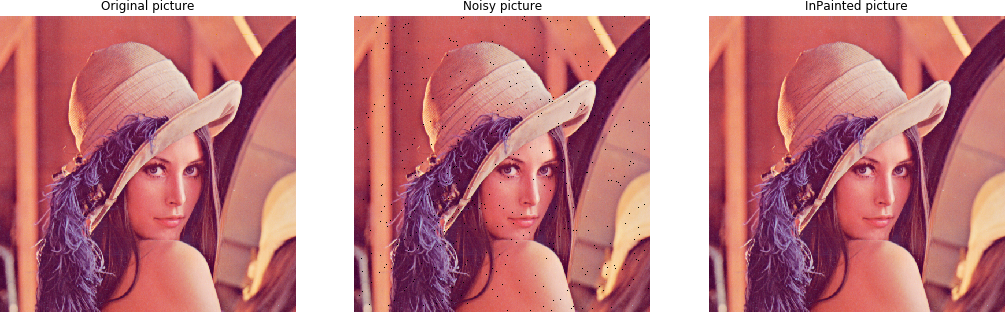
\includegraphics[scale=0.55]{res/lena_color_512_0_005.png}\\
\small{Inpainting de l'image \path{res/pictures/lena_color_512.tif}, $0.5\%$ de l'image bruitée.}
\end{center}
\begin{center}
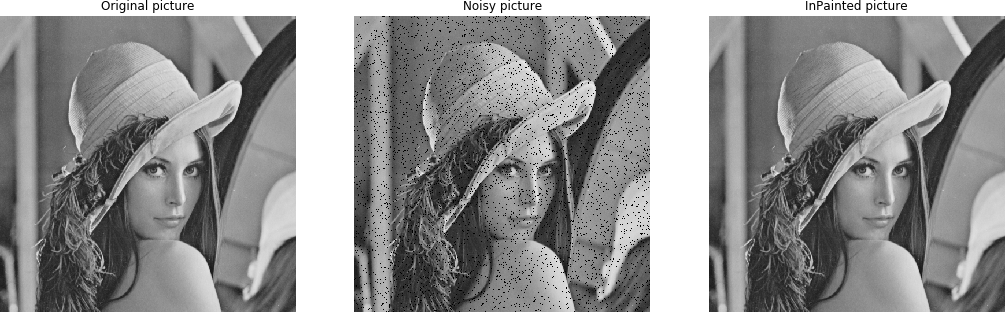
\includegraphics[scale=0.55]{res/lena_gray_512_0_05.png}\\
\small{Inpainting de l'image \path{res/pictures/lena_gray_512.tif}, $5\%$ de l'image bruitée.}
\end{center}
\begin{center}
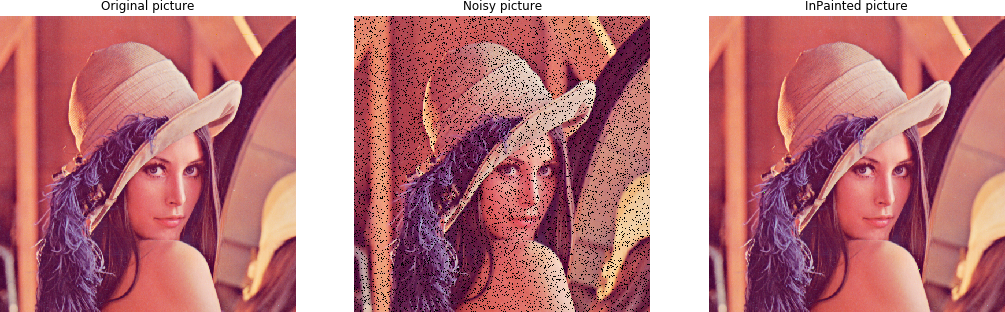
\includegraphics[scale=0.55]{res/lena_color_512_0_1.png}\\
\small{Inpainting de l'image \path{res/pictures/lena_color_512.tif}, $10\%$ de l'image bruitée.}
\end{center}
\begin{center}
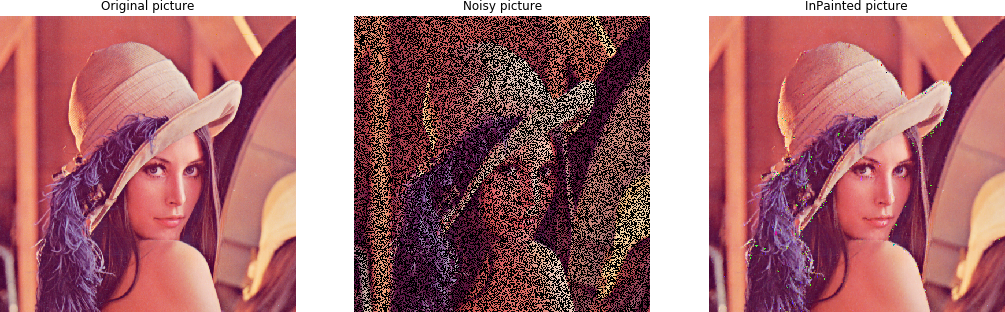
\includegraphics[scale=0.55]{res/lena_color_512_0_5.png}\\
\small{Inpainting de l'image \path{res/pictures/lena_color_512.tif}, $50\%$ de l'image bruitée.}
\end{center}

Nous obtenons des résultats visuellement très satisfaisants sur des pixels isolés. Et ce sans trop s'attarder sur les paramètres. Une petite taille de patch est cependant nécessaire pour des images beaucoup bruitées. On remarque aussi la difficulté d'approximer des détails non-redondants de l'image (l’extérieur des plumes, le contour du visage).


\newpage
\subsection{Résultats sur des patchs manquants}
La reconstruction d'une plus grosse partie d'une image devient un peu plus compliquée. En effet, les patchs à reconstituer étant de taille plus importante, nous disposons de moins d'information pour chaque patch. Il va alors falloir s'y reprendre à plusieurs fois pour trouver de bons paramètres. Testons sur l'image \path{res/pictures/outdoor.jpg} :

\begin{center}
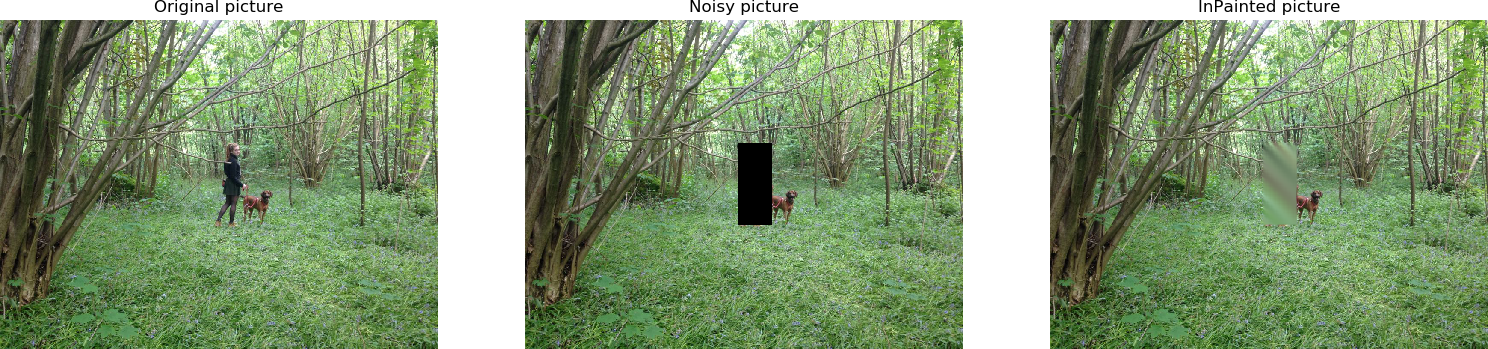
\includegraphics[scale=0.4]{res/outdoor_gros_alpha.png}\\
\small{Ici, $\alpha=0.5$, ce qui est trop gros. On effectue une combinaison linéaire avec trop de patchs, ce qui explique cet effet de flou.}
\end{center}

\begin{center}
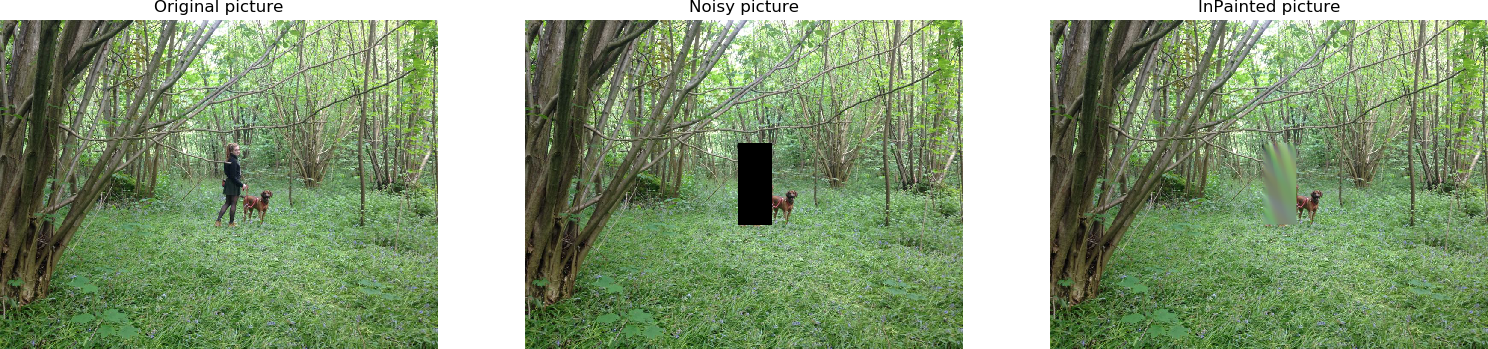
\includegraphics[scale=0.4]{res/outdoor_petit_patch.png}\\
\small{Ici, $patch\_size=5$, ce qui est trop petit. Les patchs ne contiennent pas assez d'information pour être correctement reconstruit. De plus, les pixels qui viennent juste d'être approximé sont trop pris en compte, ce qui donne un effet un peu ``baveux''.}
\end{center}


\begin{center}
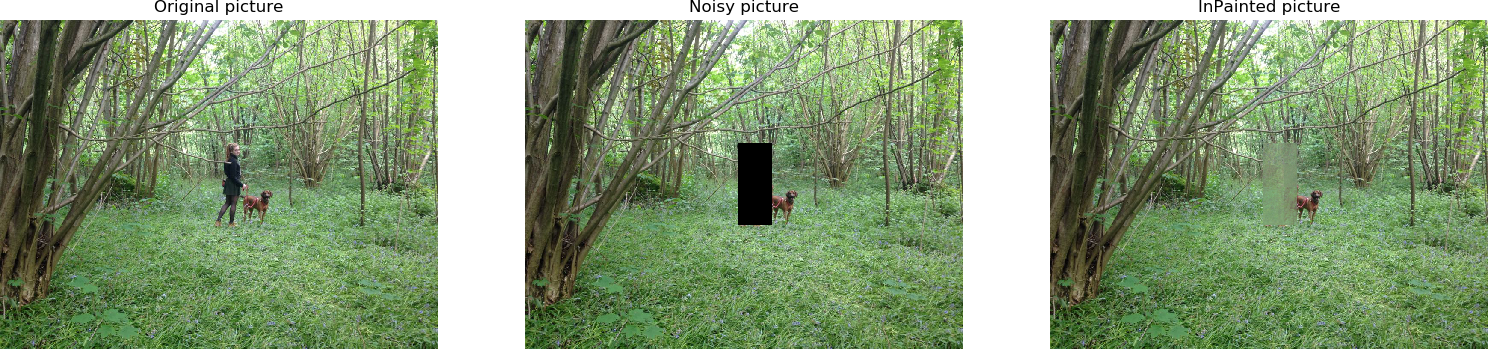
\includegraphics[scale=0.4]{res/outdoor_peu_iter.png}\\
\small{Ici, $max\_iterations=1000$, ce qui est trop peu. On dépasse ce seuil avant d'avoir trouvé les poids optimaux pour notre reconstruction.}
\end{center}


\begin{center}
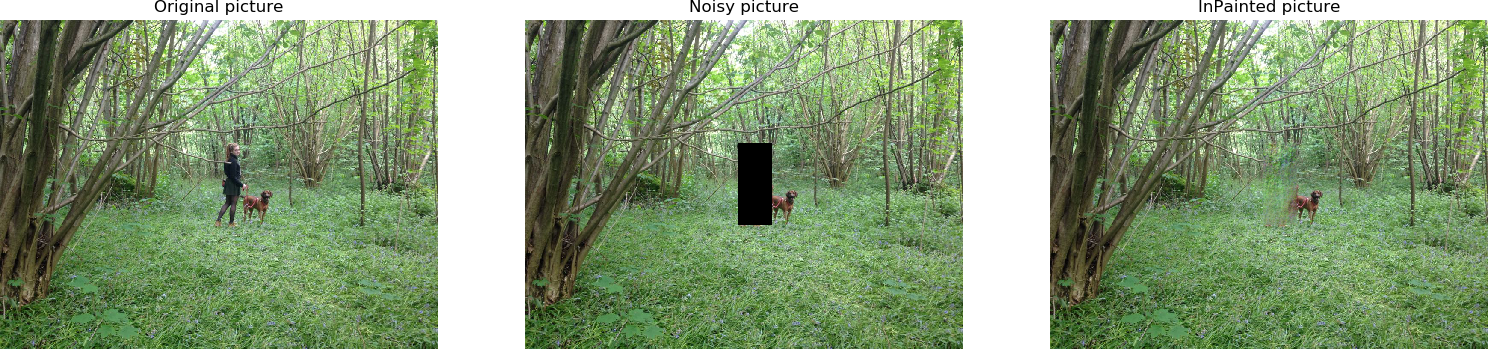
\includegraphics[scale=0.4]{res/outdoor_parfait.png}\\
\small{Ici, $\alpha=0.0001,\; patch\_size=101,\; max\_iterations=100.000$. La reconstruction parait visuellement correcte, mais elle peut sûrement être encore améliorée.}
\end{center}


\newpage
\subsection{De l'importance dans l'ordre de remplissage}
L'ordre dans lequel on choisit de remplir les patchs à toute son importance. En effet, nous utilisons un remplissage naïf de gauche à droite et de haut en bas. Ceci entraîne cependant une espèce de ``bavure'' (comme dans la deuxième figure obtenue). Ce résultat est décrit dans le papier de recherche $[3]$ donné en référence dans l'énoncé : Nous venons de reconstruire une forme particulière (comme un tronc d'arbre), et en remplissant les pixels juste en dessous à l'itération suivante, nous prendrons trop en compte les pixels que nous venons de reconstruire.\\
Voici une manière efficace pour remplir un trou :\\
Tout d'abord, assigner une valeur de \textbf{priorité} à chaque patch. Plus elle est haute, plus il faudra traiter ce patch en premier. On peut décompenser cette priorité en un \textit{produit de deux valeurs} : un coefficient d'\textbf{information}, indiquant à quel point un patch est proche de pixels purs, et un coefficient \textbf{isophotique}, caractérisant la force des \textit{isophotes} (la direction et l'intensité des pixels) autour du patch.\\
Grossièrement, cette heuristique permet de reconstruire en premier lieu les contours du trou, tout en priorisant les gros changements d'intensité autour du trou (souvent liés à une coupe perpendiculaire au trou).


\end{document}
